\documentclass{beamer}
\usepackage{listings}
\lstset{
%language=C,
frame=single, 
breaklines=true,
columns=fullflexible
}
\usepackage{subcaption}
\usepackage{url}
\usepackage{tikz}
\usepackage{tkz-euclide} % loads  TikZ and tkz-base
%\usetkzobj{all}
\usetikzlibrary{calc,math}
\usepackage{float}
\newcommand\norm[1]{\left\lVert#1\right\rVert}
\renewcommand{\vec}[1]{\mathbf{#1}}
\usepackage[export]{adjustbox}
\usepackage[utf8]{inputenc}
\usepackage{amsmath}
\usetheme{Boadilla}

\usetkzobj{all}

\title{ Problems On Geometry Of Circle}
\author{Yogesh Choudhary}
%\institute{Indian Institute of Technology, Bhilai.}
\date{\today}
\begin{document}
	\begin{frame}
		\titlepage
	\end{frame}
	\section{Question}
	
	
		\begin{frame}
			\frametitle{Question}
			\begin{block}{Exercise 8.5(Q no.13)}
				If a line segment joining two points subtends equal angles at two other points lying on the same side of the line containing the line segment, the four points lie on a circle.
			\end{block}
		\end{frame}
	
	

	\section{\textbf{Construction}}
	\subsection*{Codesandfigures}
	\begin{frame}[fragile]
		\frametitle{Codes and Figures}
		\tiny
		\begin{flushleft}
		The python code for the figure is
			\begin{lstlisting}
				./code/c_circle.py
			\end{lstlisting}
		The latex- tikz code is
			\begin{lstlisting}
				./figs/C_circle.tex
			\end{lstlisting}
		The above latex code can be compiled as standalone document
			\begin{lstlisting} 
				./figs/C_circle_fig.tex
			\end{lstlisting}
		\end{flushleft}.
%\begin{columns}
%\column{0.5\textwidth}
		\begin{figure}
			\begin{minipage}{0.45\linewidth}
			\begin{subfigure}{0.5\textwidth}
			\begin{flushleft}
				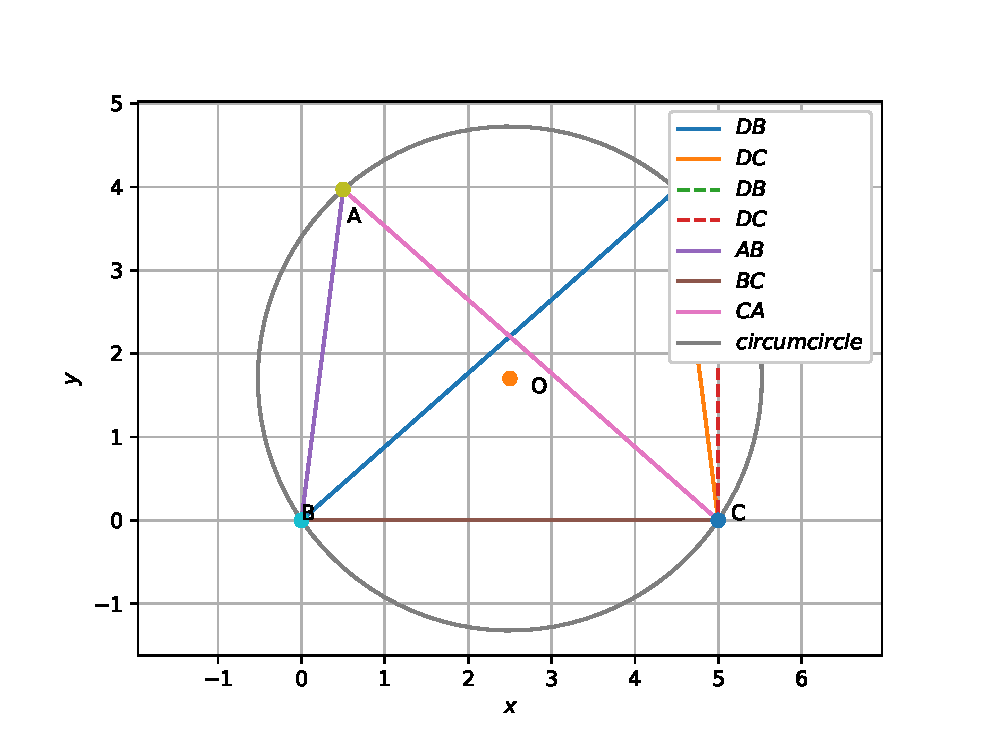
\includegraphics[scale=0.3]{./figures/c_circle.eps}
				\caption{\tiny By Python}
			\end{flushleft}
			\end{subfigure}
			\end{minipage}
			\hfill
			\begin{minipage}{0.45\linewidth}
			\begin{subfigure}{0.5\textwidth}
			\begin{flushright}
				\resizebox{1.3\columnwidth}{!}{	\begin{tikzpicture}
[scale=2,>=stealth,point/.style={draw,circle,fill = black,inner sep=0.5pt},]

%Triangle sides
\def\a{5}
\def\b{6}
\def\c{4}
\def\R{3.023715784073818}

%Coordinates of A
%\def\p{0.5}
\def\p{((\a^2+\c^2-\b^2)/(2*\a))}
\def\q{{sqrt(\c^2-\p^2)}}

\def\x{((\a^2+\b^2-\c^2)/(2*\a))}
\def\y{{sqrt(\b^2-\x^2)}}

%Labeling points
%\node (A) at ($({((\a^2+\c^2-\b^2)/(2*\a))},{sqrt(\c^2-\x^2)} )$)[point,label=above right:$A$] {};
\node (A) at ($({((\a^2+\c^2-\b^2)/(2*\a))},{sqrt(\c^2-\p^2)} )$)[point,label=below left:$A$] {};
\node (B) at (0, 0)[point,label=below left:$B$] {};
\node (C) at (\a, 0)[point,label=below right:$C$] {};
\node (D) at ($({((\a^2+\b^2-\c^2)/(2*\a))},{sqrt(\b^2-\x^2)} )$)[point,label=below left:$D$] {};
%\node (E) at ($({(\a)}, {((\a)/((\a^2+\b^2-\c^2)/(2*\a))*(sqrt(\c^2-\p^2))})$)[point,label=below right:$E$] {};
%Circumcentre

\node (O) at (2.5,1.70084013)[point,label=above right:$O$] {};

%Drawing triangle ABC
\draw (A) -- node[left] {$\textrm{c}$} (B) -- node[below] {$\textrm{a}$} (C) -- node[above,yshift=2mm] {$\textrm{b}$} (A);

\draw (D) -- node[left] {$\textrm{e}$} (B);
\draw (D) -- node[left] {$\textrm{d}$} (C);

%\draw[dashed] (E) -- node[left] {$\textrm{}$} (B);
%\draw[dashed] (E) -- node[left] {$\textrm{}$} (C);
%Drawing OA, OB, OC
%\draw (O) -- node[left] {$\textrm{R}$} (A);
%\draw (O) -- node[below] {$\textrm{R}$} (B);
%\draw (O) -- node[below] {$\textrm{R}$} (C);
\draw (O) circle (\R);

%\tkzMarkAngle[fill=blue!50,size=.3](C,B,A)
%\tkzMarkAngle[fill=blue!50,size=.3](O,C,B)


%\tkzMarkAngle[fill=red!50](O,A,C)
\tkzMarkAngle[fill=red!50,size=.3](B,D,C)
%\tkzMarkAngle[fill=red!50,size=.3](B,E,C)

\tkzMarkAngle[fill=orange!50,size=.3](B,A,C)
%\tkzMarkAngle[fill=orange!50,size=.3](O,B,A)
\tkzMarkAngle[fill=red!50,size=.3](B,D,C)
\tkzMarkAngle[fill=red!50,size=.3](C,B,D)
\tkzMarkAngle[fill=red!50,size=.3](D,C,B)
%\tkzLabelAngle[pos=0.5](A,C,B){$\theta_1$}
%\tkzLabelAngle[pos=0.5](O,B,C){$\theta_1$}
\tkzLabelAngle[pos=0.5](B,D,C){$\theta_2$}
%\tkzLabelAngle[pos=0.5](B,E,C){$\theta_3$}

\tkzLabelAngle[pos=0.5](B,A,C){$\theta_1$}
%\tkzLabelAngle[pos=1.5](O,C,A){$\theta_3$}
\tkzLabelAngle[pos=0.5](C,B,D){$\beta_2$}
\tkzLabelAngle[pos=0.5](D,C,B){$\alpha_2$}

	
	\end{tikzpicture}
	}
				\caption{\tiny By Latex-tikz}
			\end{flushright}
			\end{subfigure}
			\end{minipage}
			\end{figure}
		\end{frame}
	
		
		
	\subsection*{Construction methods}
	\begin{frame}[fragile]
	\footnotesize
	\frametitle{Construction method}
	\begin{columns}
		\begin{column}{0.5\textwidth}
			A circumecircle is to be made having two triangles with vertices on the circle and a point $\vec{e}$ outside of the circle,with the help of the three sides of a triangle as input as shown in the table below.
			
		\begin{table}[htbp]
		\centering
  		\resizebox{1\textwidth}{!}
  		{\begin{minipage}{\textwidth}
			\begin{tabular}{ |p{2cm}|p{2cm}|  }
			\hline
 			\multicolumn{2}{|c|}{Initial Input Values.} \\
			\hline
			a & 5\\
			\hline
			b & 4\\
			\hline
			c & 6\\
			\hline
			\end{tabular}
		\end{minipage}}
		\caption{\tiny To construct the circumecircle}
		\end{table}
	\end{column}

	\begin{column}{0.5\textwidth}
	Finding out the all points given in the figures 
	\newline
	$$(i)\vec{A}= \begin{pmatrix}0.5\\3.968\end{pmatrix}
	(ii)\vec{B}=\begin{pmatrix}0\\0\end{pmatrix}$$
	\\
	$$(iii)\vec{C}=\begin{pmatrix}5\\0\end{pmatrix}
	(iv)\vec{D}= \begin{pmatrix}4.5\\3.98\end{pmatrix}$$
	$$(v)\vec{E}=\begin{pmatrix}5\\4.40\end{pmatrix}$$
	\end{column}
\end{columns}
\end{frame}





\section*{\textbf{Solution}}
\begin{frame}[fragile]
\footnotesize
\begin{columns}
\begin{column}{0.5\textwidth}
	Now,calculating circumecentre of the triangle
	\\ 
	$$\norm{\vec{A}-\vec{O}}^2 - \norm{\vec{B}-\vec{O}}^2 = 0$$
	\\
	Which can be simplified as
	$${\begin{pmatrix}\vec{A}-\vec{B}\end{pmatrix}}^T \vec{O} = \frac{(\norm{A}^2 -\norm{B}^2)}{2}$$

	Similarly,

	$${\begin{pmatrix}\vec{B}-\vec{C}\end{pmatrix}}^T \vec{O}  = \frac{(\norm{B}^2 -\norm{C}^2)}{2}$$
   Above equation can be combinrd as $\to$
   \\
   $$\vec{O} = \vec{N}^{-T} \vec{c}$$
	Where
	\begin{equation}
	\vec{N} = \begin{pmatrix}\vec{A} -\vec{B} & \vec{B}-\vec{C}\end{pmatrix}
	\end{equation}
	\end{column}

	\begin{column}{0.5\textwidth}
	$$\vec{c} = \frac{1}{2}\begin{pmatrix}\norm{A}^2 -\norm{B}^2 \\ \norm{B}^2 - \norm{C}^2\end{pmatrix}$$
	Finding out the $\vec{R}$
	\\
	$$\vec{R} = \norm{\vec{B}- \vec{O}}$$
	\\
	$$\vec{R} = 3.023$$
	
	\begin{table}[H]
	\centering
	\resizebox{1\textwidth}{!}
	{\begin{minipage}{\textwidth}
		\begin{tabular}{ |p{2cm}|p{2cm}|  }
			\hline
			\multicolumn{2}{|c|}{Derived Values for $triangle DCB$.} \\
			\hline
			\centering
			$\vec{O}$ & $$\begin{pmatrix}2.5\\1.70\end{pmatrix}$$\\	\hline
			\end{tabular}
	\end{minipage}}
	\caption{\tiny circumecentre of the triangle}
\end{table}
\end{column}
\end{columns}
\end{frame}



\section*{\textbf{Solution}}
\begin{frame}[fragile]
	\footnotesize
	\frametitle{Solution)}
	\begin{columns}
		\begin{column}{0.5\textwidth}
			Let assume that  circle intersect at $\vec{E}$
			\\
			Now,
			\\
			$$\angle{BAC} = \angle{BEC}$$
			(Angle in the same segment are equal)
			\\
			But given that
			\\
			$$\angle{BAC} = \angle{BDC}$$
			\\
			So from above equations 
			$$\angle{BEC} = \angle{BDC}$$
			\\
		\end{column}
		\begin{column}{0.5\textwidth}
			From the triangle DEC
			$$\angle{BDC} = \angle{CED} + \angle{DCE}$$
			(Exterier angle property of triangle)
			\\
			$$\angle{BEC} = \angle{BEC} + \angle{DCE}$$
			\\
			$$\angle{BEC} - \angle{BEC} = \angle{DCE}$$
			\\
			$$\angle{DCE} = 0$$
			From above we can say that can not exist out of the periphery of the circle 
		\end{column}
	\end{columns}
\end{frame}

\end{document}
